\section{Correlation between Submission Properties and Detection Rate}
\label{sec:corr}
Detection rate is what most \vt\ users refer to decide whether their submissions
are benign or malware and the first thing that a user of \vt\ uses. 
Therefore, it is important to study what factors affect or correlate to detection rates. 

While anti-virus engines detect malware relying on the direct analysis of files themselves, 
scanning and analyzing the large amount of files can be time-consuming and require lots of computing resources, 
especially in today's big-data era.
Moreover, obtaining original files may not always be possible or desirable;
for example, users may not want to disclose their files to an online service like \vt\ but still want to detect malware in their files.
Thus, we raise the question of {\em if there is any way to assist or even conduct malware detection with file properties only?}

%The results provide a mechanism to guide security researchers 
%and vendors to have targeted investigation over
%{\em suspicious} files, 
%files that have the factors that we identify as highly correlated to detection rate.

This section presents our study of the correlation between various properties of
\pe\ submissions and their detection rate. 
We focus on \vt\ submissions' properties that can be obtained without executable binary files
%We studied a range of properties 
and studied their correlation with detection rate.
We found that three factors have higher correlation:
submission file size,
historical submission properties, and the reputation of source IDs.
We also built a regression model based on these three factors to predict detection rate.
We present these correlation study results and our regression model in this section.
%In the next section, we will present our further analysis of what can affect the detection result of anti-virus engines
%and if detection rate is a perfect measurement of the likelihood of malware.


%\begin{figure}[t!]
\begin{center}
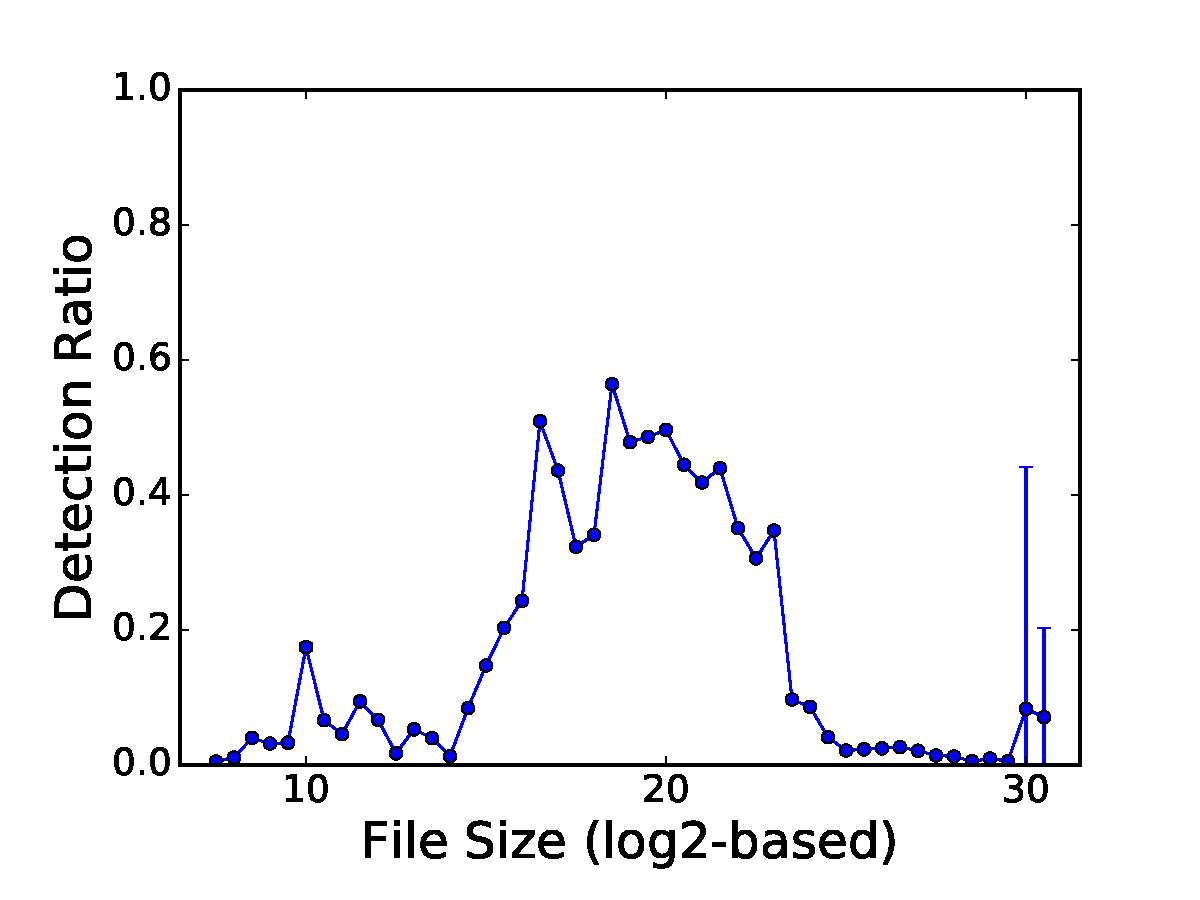
\includegraphics[width=2in]{figure/size}
  \caption{How detection rate changes with file size.
(
95\% confidence interval is also drawn for each point.
Results of log2 for the original file sizes are rounded to the nearest 0.5 value.)
}
\label{fig:size}
\end{center}
%\vspace{-0.25in}
\end{figure}


\subsection{File Size}
\label{sec:size}
Anecdotally, \pe\ malware are most likely to have small to medium size. 
To verify this hypothesis, we analyzed the relationship between submission file size and detection rate. 
Figure~\ref{fig:size} presents the average detection rate and 
the 95\% confidence interval for different file sizes.
A wider confidence interval implies that
the calculated average detection rate is farther away from the real average detection rate.
To simplify calculation, we use discrete file sizes of powers of two in our analysis and in this graph,
i.e., we calculate the log2 of each original file size and round it to the nearest 0.5 value.
Overall, we find that files with size from 90KB to 4MB have higher detection rate, more than 20\% on average. 
Except for the last two points which represent a small amount of files that are bigger than 1GB, 
all other sizes have high confidence.   

{\bf Observation 4:} 
{\em \pe\ malware are mostly likely to be of small to medium size.}

An immediate question that follows is whether the high detection rate of files with small to medium size
is because these files also contribute to most of the submissions as shown in Figure~\ref{fig:pesize}.
As we will discuss in Section~\ref{sec:history}, the correlation of submissions and detection rate is more complex and non-linear.
Thus, there is a more fundamental reason behind the file size correlation with detection rate.
One likely reason of this correlation is that files that are too small are not enough to express the
malware functions while files that are too big are difficult to spread. 

\subsection{Submission History}
\label{sec:history}

%

\begin{figure}[t!]
\begin{center}
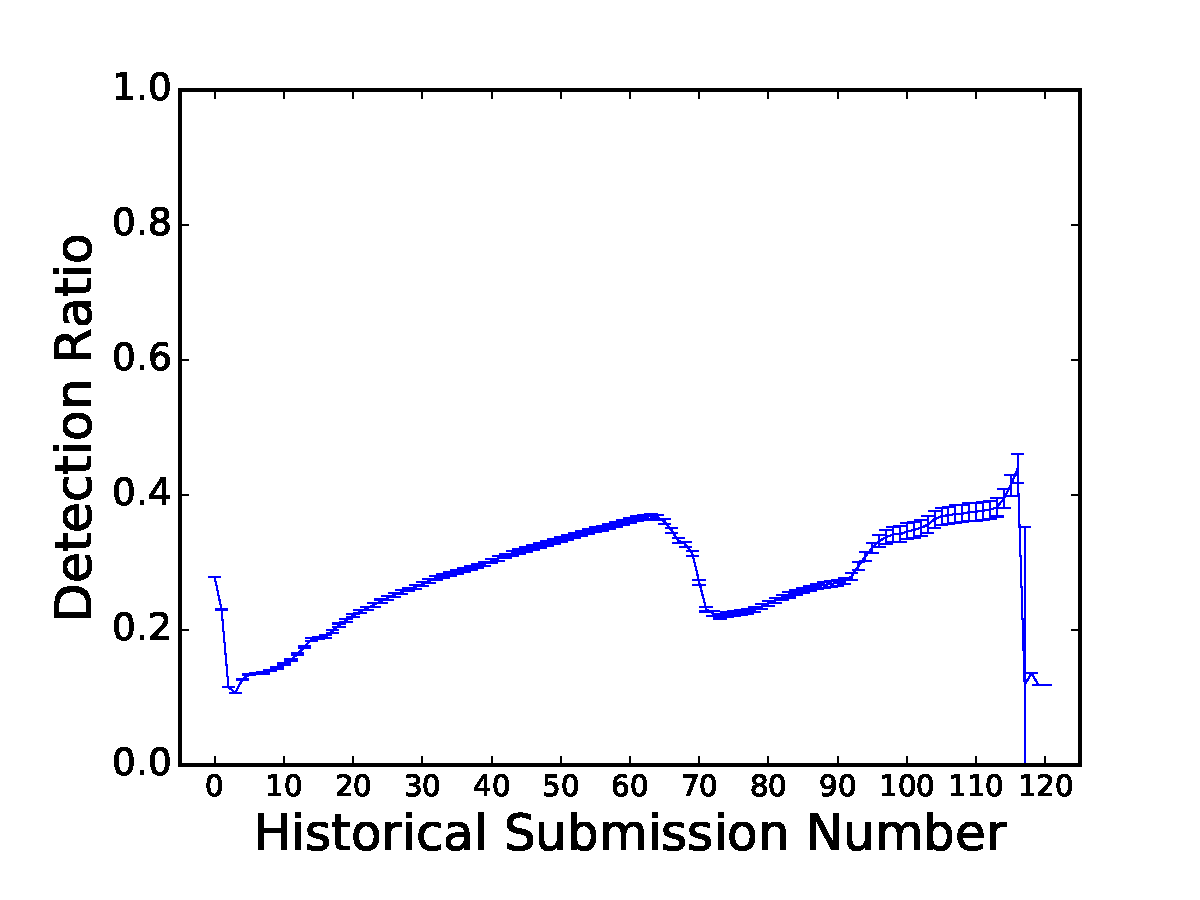
\includegraphics[width=2in]{figure/SubNum}
\caption{
The relation between historical submission number and detection rate.
(
How detection rate changes with historical submission number. 
Each historical submission number is rounded up to nearest 5.
95\% confidence interval is also drawn for each point.
)	
}
\label{fig:hisnum}
\end{center}
%\vspace{-0.25in}
\end{figure}

%\begin{figure}[t!]
%\begin{center}
%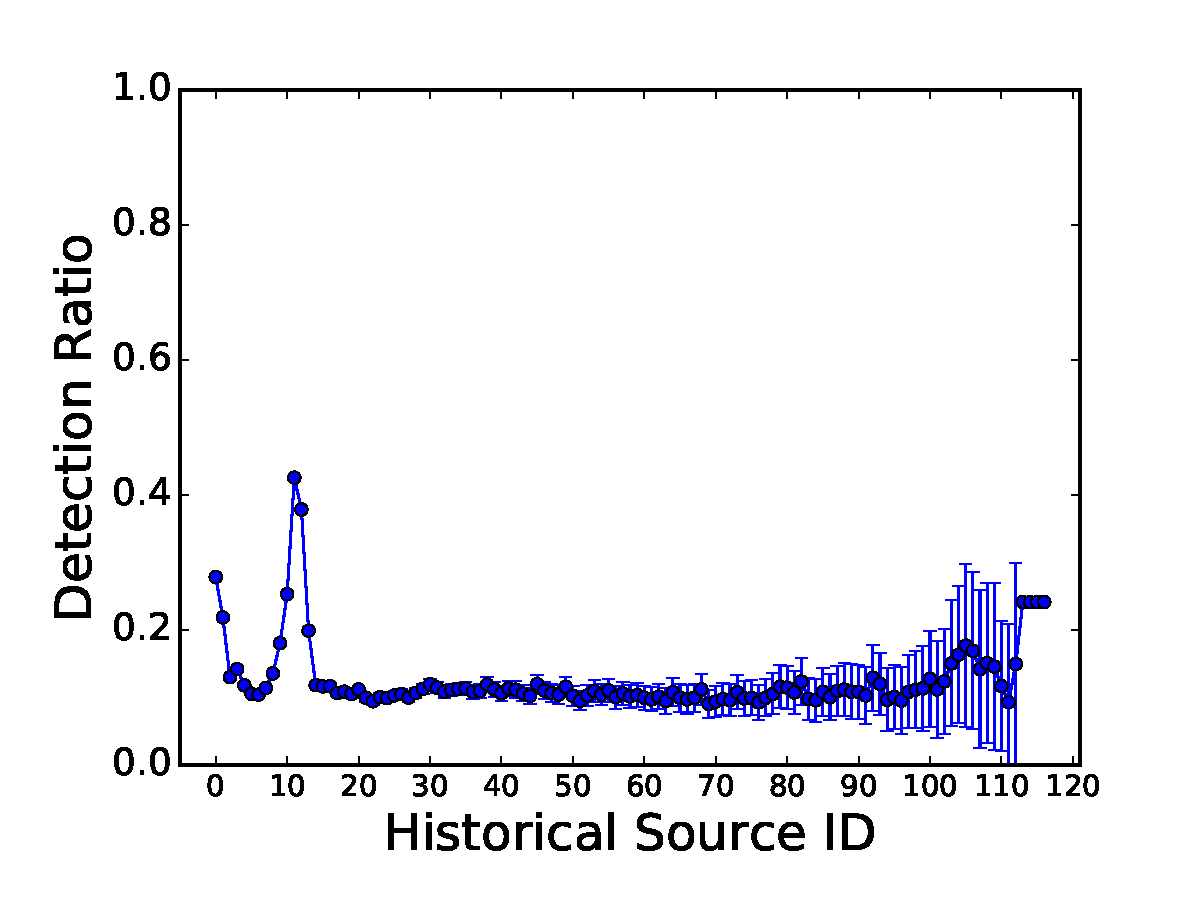
\includegraphics[width=2.5in]{figure/SubID}
%  \mycaption{fig:hisid}{The relation between the number of historical source ids and detection rate.}
%{\footnotesize{(How detection rate changes with the number of historical source ids. 
%Each historical number of source ids is rounded up to nearest 5.
%95\% confidence interval is also drawn for each point.)}}

%\end{center}
%\vspace{-0.25in}
%\end{figure}


As discussed in Section~\ref{sec:basicanal}, many files are submitted multiple times, from one or more users to VirusTotal. 
It is worthwhile to investigate this {\em history of submission} to check how history affects future.
We study the correlation between submission history and the detection rate of the current submission.
Among the different types of historical information that we study including the number of submissions of a file made in history, the number of users that submitted the same file in history, and the number of countries that have submitted a file,
we find that the number of submissions made in history has the highest correlation to detection rate.

%\noindent{\textit{\underline{The number of submissions in history.}}}
To study the submission history, we first sort all submissions for each file chronologically
and then collect the number of all submissions made before submission $s$ for each submission $s$ in \vt.
Next, we calculate the correlation between detection rate and the number of submission in history.
Figure~\ref{fig:hisnum} plots how detection rates change over the number of historical submissions.

The overall trend from this result is that more historical submissions result in higher detection rate.
Intuitively, if a file is submitted many times, it means that many users suspect this file as malware
and/or a user insist her suspicion that the file is malware and submit it over and over.
In both cases, there is a higher chance that this file indeed is malware and is thus being detected as malware by more anti-virus engines.

Interestingly and counter-intuitively, there are three drops in the beginning, middle, and end. 
We think that for files with high detection rate, users are satisfied with \vt{}'s results, 
and they stop submitting these files. 
Percentage of submitted files with low detection rate increases, and this causes average detection rate drops. 

%{\color{red} I don't fully understand and buy your following explanation and come up with the above explanation for the increasing range.
%But I still don't know how to explain the drops. Can you think about it?}

\if 0
To explain this effect, we look at the two factors that can both influence detection rates:
the percentage of benign files submitted and the amount of anti-virus engines labeling the submission as malware.
%Two factors can influence detection rates and explain the above effect.
Obviously, with more benign files submitted, detection rate will decrease
and with more engines labeling malware, detection rate will increase. 
In the the two stages of detection rate increasing (from 1 to ~60 and from~70 to ~115 {\color{red} fill with exact numbers}), 
with more submissions, more engines are able to identify malware 
and the increase of percentage of engines identifying submitted malware dominates. 
In the range that detection rate drops (from ~60 to ~70 {\color{red} fill with exact numbers}), 
VirusTotal users stop submitting files that have already been identified as malware,
and the increase of percentage of benign files submitted to VirusTotal dominates. 
\fi

{\bf Observation 5:} 
{\em The number of submissions made in history has some correlation with detection rate, 
but the correlation is non-linear and is affected by multiple factors.}

\subsection{Submitting User}
\label{sec:reputation}



\begin{figure}[t!]
\begin{center}
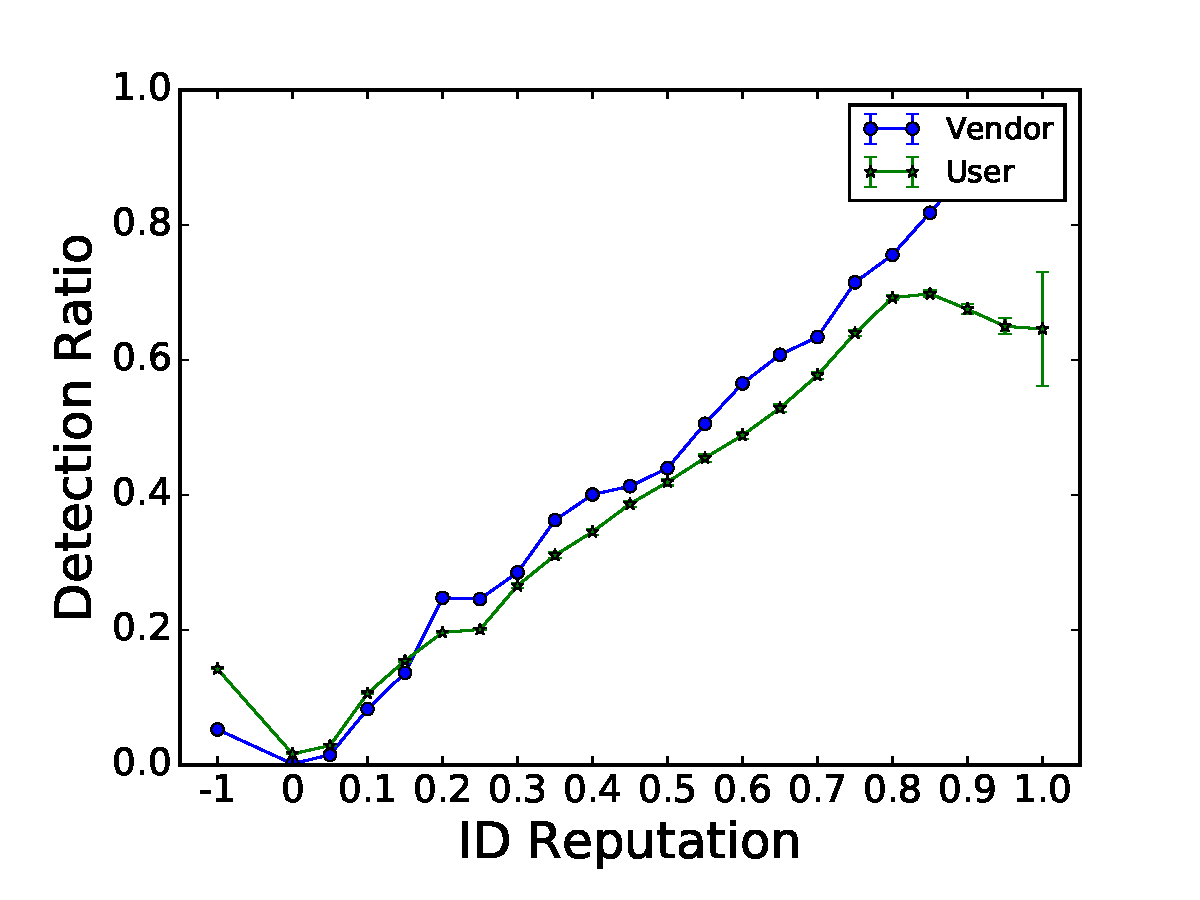
\includegraphics[width=2in]{figure/IDReputation}
\caption{The relation between source id's previous reputation and detection rate.
(How detection rate changes with the value of source id's reputation. 
Each reputation is rounded up to nearest 0.05.
Reputation -1 means the source id did not make any submission before. 
95\% confidence interval is also drawn 
for each point.)
}
\label{fig:idreputation}
\end{center}
%\vspace{-0.25in}
\end{figure}

Different users of online services such as \vt\ often have different {\em reputation} 
because of different motivations, objectives, and backgrounds.
For example, some users can randomly trying out \vt\ with no specific objective and thus submit random files,
while other users have clear goals and motivations and thus only submit suspicious files.
The rationale behind reputation is that \vt{} users would have a roughly constant submission pattern, 
and it is promising to use their historical submission to predict their future submission.
Previous work~\cite{GuoICSE2010} reported that there is a correlation between bug reporter's reputation and the likelihood for the bug being fixed. 
We also observe correlation between the reputation of source ID and submission's detection rate. 

Intuitively, a user that have submitted more files that were detected as malware suggest 
that she is more likely to use \vt\ to detect malware in suspicious files 
and thus should be given higher reputation.
The reputation of a source ID is not a fixed value and can change over time. 
To quantify this value, we define the reputation of a source ID, the unique identifier of a \vt\ user, as the follow.

%\theoremstyle{definition}
\begin{definition}{Reputation:}
Given a submission $S$ with source ID $N$, 
we define the reputation of $N$ when conducting the submission $S$ as the average detection rate for all submissions conducted by $N$ before $S$. 
If $N$ did not make any submission before, we define the reputation to be $-1$. 
\end{definition}

Before conducting our source ID reputation analysis, we first filter out submissions
that have no source ID information and submissions by source IDs with more than 1 million submissions (these are likely to be bogus or coming from robots).
For the remaining source IDs, we then sort submissions from the same source ID chronologically 
and calculate each source ID's reputation when it conducts a submission. 
We further separate normal users from vendors and analyze the correlation of their ID reputation and detection rate.

Figure~\ref{fig:idreputation} plots the average detection rate and the 95\% confidence interval 
as the source ID reputation increases for normal users and for anti-virus vendors.
We round up reputation values to their nearest 0.05 values. 

Detection rate steadily increase as the reputation increases from 0 to 1 for vendors and from 0 to 0.8 for normal users.
Except the points when reputation is 1, all other results have high confidence.
Interestingly, for both normal user and vendors the detection rate with reputation -1 is higher than with reputation 0,
which means that the first submissions conducted by all source IDs (reputation -1) 
generally have higher detection rate than 
the submissions conducted by IDs that have only submitted benign files (reputation 0).

For normal users, the detection rate drops when reputation is greater than 0.8,
which means that for normal users, it is difficult for them to always submit suspicious files detected by almost all vendors.
Vendors do not exhibit this behavior and their detection rate always increases with higher reputation (other than reputation -1),
showing that vendors' reputation can almost always be trusted.


{\bf Observation 6:} 
{\em There is a high correlation between user reputation and detection rate of their submissions for both normal users and anti-virus vendors.}


\subsection{Comprehensive Correlation Model}

From the above study in this section, we find three factors that are correlated to detection rate: 
submission file size, the number of submission made in history, and source ID reputation.
Two natural questions that follow are {\em how the combination of these three factors correlate to detection rate} and 
{\em whether or not we can use these finding to predict the likelihood of a file being malware}.
A positive answer to the second question can largely assist security researchers and practitioners to narrow down 
the vast suspicious files to a much smaller set.
More important, such an answer can open up the possibility to perform an initial prediction of malware {\em with metadata only} and 
{\em no original file}.

\noindent{\underline{\textit{Methodology.}}}
To answer these questions, we build a linear regression model using the three factors as features of the model 
to predict the detection rate of a submission.   
We first filter out submissions without source ID reputation information (Section~\ref{sec:reputation}). 
We then randomly divide remaining submissions into a training set and a testing set with equal size. 
We use training set to train our regression model and two ways for testing the trained model:
in-sample testing where we use the whole training set for testing, and out-of-sample testing where we use the testing set for testing. 

For comparison to our regression model, we use a model that is based on random guesses;
it guesses the detection rate for any submission 
as the mean of detection rate for all training submissions. 

We calculate the mean absolute error ({\em mae})~\cite{mae} 
and the mean squared error ({\em mse})~\cite{mse} to compare our regression model and the random model. 
Smaller mae and mse values mean lower error rates. 

\noindent{\underline{\textit{Modeling results.}}}
For in-sample testing, mae and mse for our regression model are 0.2227 and 0.0718 respectively, 
while for baseline model they are 0.3345 and 0.1327. 
For out-of-sample testing, mae and mse for our regression model is 0.2223 and 0.0716 respectively, 
and they are 0.3342 and 0.1325 for baseline model. 
For both in sample testing and out of sample testing, our regression model %significantly 
improves the prediction accuracy over the random model (from 33.4\% to 46.0\%).
%{\color{red} check if this is significant}
Errors of our regression model under in-sample testing and out-of-sample testing are almost the same, 
which shows that our model generalizes well across different data set. 

After obtaining satisfactory accuracy results with our regression model above, 
we further analyze the importance of each of the three factors in achieving good model accuracy.
The learned coefficients from our regression model for submission file size, the number of submission made in history, and source ID reputation 
are $7.12 * 10^{-3}$, $1.76 * 10^{-4}$, and $6.03 * 10^{-1}$ respectively. 
To understand the impact of each factor on prediction results, 
we exclude the three factors one by one and use the remaining two to train 
three regression models with out-of-sample testing. 
Excluding submission file size, the number of submissions in history, and source ID reputation increase mse 
to 0.0844, 0.716, 0.1390 respectively (17.9\%, 0\%, 94.1\% worse), 
%and removing the number of submission increases mse less than $10^{-4}$. 
This result shows that source ID reputation has the biggest influence on detection rate, 
while the number of submissions in history has insignificant influence.
There are two possible reasons why the number of submission in history has only a very small influence on detection rate. 
First, the majority of files are only submitted once in \vt. Thus, all these submissions have the same number of submission made in history, but have various detection rate. 
Second, the relationship between the number of submission and detection rate is not linear as shown in Figure~\ref{fig:hisnum}.
Thus, only one coefficient cannot describe how detection rate change with the number of submission precisely. 


{\bf Observation 7:} 
{\em Regression model built with the three studied factors can help the prediction of detection rate for malware submissions. 
Among these three factors, source ID reputation has the most significant impact on detection rate, while the number of submissions 
made in history has only a minimal impact.}


\subsection{Discussion}

From our analysis, file size, number of submissions in history, 
and source ID reputation are all correlated with detection rate.
Our regression model based on these three factors can effectively help predict detection rate for \vt\ submissions. 

All the three studied factors can be obtained without analyzing binary executable files.
These factors plus our regression model provide an easy way to
perform an estimated malware prediction of a file without knowing the file content.  
Researchers and vendors can use this method to perform an initial filtering of the huge amount of malware submissions, 
so that they can easily focus on more interesting files---files that are more likely to be malicious.
More important, our results here shed light on the possibility 
for normal users to not disclose their files while still 
be able to have an initial prediction of suspicious files.
%Anti-virus vendors can also inspect results which are variant from our prediction results 
%to identify possible false positives or false negatives in their products. 
%File size information can be accessed in \vt~'metadata. 
%Number of submissions in history and source ID reputation are computed by ourselves. 
%Our studying results suggest that \vt\ should also track number of submissions in history for each file and reputation for each source ID in the future. 

